\documentclass[student]{ITRslides}
\usepackage{tikz,pgfplots}
\addbibresource{ref.bib}
\graphicspath{{pics/}{logos/}}


\title{Control of a multi-robot cooperative team guided by a human operator}
\presenter{M. Angerer}

\supervisor{S. Musi\'c}
\typeofpres{Intermediate Presentation Master Thesis}

\usetikzlibrary{decorations.pathreplacing}
\newcommand{\tikzmark}[2]{\tikz[remember picture,baseline=(#1.base)]{\node[inner sep=0pt] (#1) {#2};}}
%%%%%%%%%%%%%%%%%%%%%%%%%%%%%%%%%%%%%%%%%%%%%%%%%%%%%%%%%%%%%%%%%%%%%%%%%%%%%%%%

\begin{document}


\begin{frame}
    \titlepage
\end{frame}

%\begin{frame}
%	\frametitle{Overview}
%    \tableofcontents%[hideallsubsections]%[pausesections]
%\end{frame}

\section{Introduction}

\begin{frame}
	\frametitle{Why use human guided cooperative manipulation?}
		\begin{columns}[t]
		\column{0.5\linewidth}
	
			\begin{figure}
			\centering
			%\psfrag{q1}[Bl][Bl]{\small $\alpha$}
			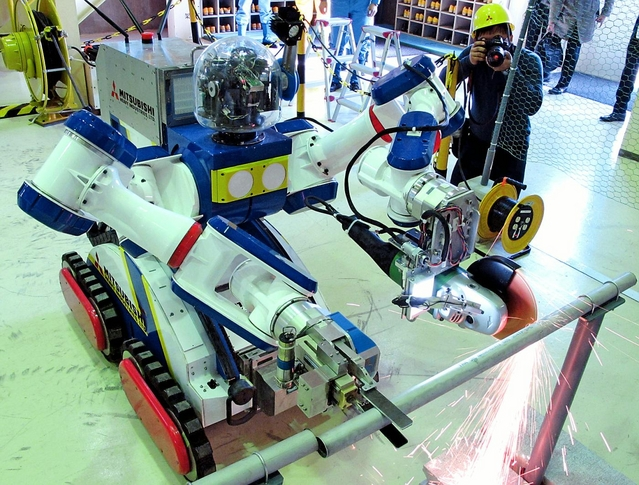
\includegraphics[width=0.98\textwidth]{mhi-meister45.jpg}
			%\caption{Coordinated handling of tools by a tele-operated robot \cite{MHI-MEISTeR}}
			\end{figure}
		
		\column{0.6\linewidth}
			
		Human reasoning
		\begin{itemize}
			\item Foresight and adaptiveness to incidents
			\item Superior planning capabilities
		\end{itemize}
		\vspace{15pt}
		Enhanced flexibility of multiple robots
			\begin{itemize}
				\item Transportation of large/heavy objects
	\item Assembly of multiple parts 
	\item Coordinated use of tools
			\end{itemize}
			
			\end{columns}
\end{frame}

\begin{frame}
	\frametitle{Problem setting}
		\begin{columns}
%	\begin{itemize}
%		\item Precise and stable control during free-motion/contact transition
%		\item Enhance versatility by performing friction grasps
%		\item (Intuitive) high-level human shared control
%		\item Local control of formation, independent of the operator
%		\item Assistance of the operator with suitable feedback
%	\end{itemize}
	\column{0.5\linewidth}
	\begin{itemize}
	\item A set of robots manipulating a common object
	\item A human guiding the formation by hand motion
	\end{itemize}
		
	\column{0.5\linewidth}
	
	
			\begin{figure}
			\centering
			%\psfrag{q1}[Bl][Bl]{\small $\alpha$}
			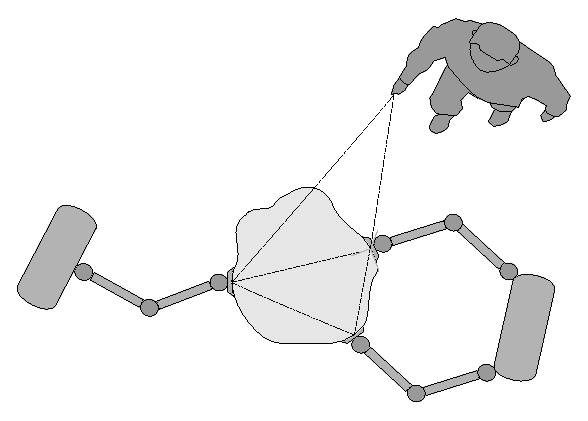
\includegraphics[width=0.8\textwidth]{general_setup.eps}

			\end{figure}
	\end{columns}
	\vspace{10pt}
	\begin{block}{Goal}
	\begin{itemize}
	\item Consistent modelling of constrained systems 
	\item Model-based control with human-in-the-loop
	\end{itemize}
	\end{block}	

\end{frame}

\begin{frame}
	\frametitle{Related Work}
	\textbf{Robot-team control}
	\begin{itemize}
		\item Virtual object based impedance control \nocite{Schneider_92} {\tiny [SC92]} 
				\item Internal and external impedance control \nocite{Caccavale_01,Caccavale_08} {\tiny [CV01,CCMV08]} 
%			\begin{itemize}
%			%\item object tracking required
%			%\item knowledge of object shape and dynamics required
%			%\item Force/Torque sensors at the manipulators required
%			\end{itemize}
	
		\item Intrinsically Passive Control \nocite{Stramigioli_01, Wimboeck_08} {\tiny [Str01,WOH08]} 
%		\begin{itemize}
%			%\item no object tracking, virtual object simulation
%			%\item knowledge of object shape and dynamics required
%		\end{itemize}
		\item Object dynamics' feed-forward \nocite{Erhart_15} {\tiny [EH15]} 
	\item Formation control of a robot team \nocite{Sieber_15,Wimboeck_06}{\tiny [SMH15,WOH06]} 
%		\begin{itemize}
%			%\item no object dynamics considered
%			%\item no knowledge of object required
%		\end{itemize}
	\end{itemize}
	\textbf{Human in the loop}
	\begin{itemize}	
		\item Formation-based control \nocite{Sieber_15, Scheggi_14}{\tiny [SMH15,SMP14]} 
%		\begin{itemize}
%			\item Single leader, multiple followers
%			\item Robots preserve formation autonomously
%			\item Tactile feedback
%		\end{itemize}
		\item Bilateral tele-manipulation  \nocite{Lee_05} {\tiny [LS05]} 
%		\begin{itemize}
%			\item Single master coupled to human, constrained system as slave
%			\item Local control of interaction dynamics
%			\item Force feedback
%		\end{itemize}

		\item Gesture-based Control \nocite{Gioioso_2014}{\tiny [GFS+14]} 
%		\begin{itemize}
%			\item Free-hand motion controls constrained system
%			\item Visual feedback
%			%\item only visual feedback
%		\end{itemize}
		\end{itemize}
		
			\begin{block}{}
			\begin{itemize}
			\item port-Hamiltonian systems allow for energy consistent modelling of complex physical systems
			\item \emph{IPC} concept based on a physical model

			\item Closed loop stability for bounded energy supply% and a passive control architecture
			\end{itemize}
			\end{block}
\end{frame}

%\begin{frame}
%	\frametitle{Related Work: Human in the loop}
%	\begin{itemize}	
%		\item Formation-based control \nocite{Sieber_15, Scheggi_14}{\tiny [SMH15,SMP14]} 
%%		\begin{itemize}
%%			\item Single leader, multiple followers
%%			\item Robots preserve formation autonomously
%%			\item Tactile feedback
%%		\end{itemize}
%		\item Bilateral tele-manipulation  \nocite{Lee_05} {\tiny [LS05]} 
%%		\begin{itemize}
%%			\item Single master coupled to human, constrained system as slave
%%			\item Local control of interaction dynamics
%%			\item Force feedback
%%		\end{itemize}
%
%		\item Gesture-based Control \nocite{Gioioso_2014}{\tiny [GFS+14]} 
%%		\begin{itemize}
%%			\item Free-hand motion controls constrained system
%%			\item Visual feedback
%%			%\item only visual feedback
%%		\end{itemize}
%		\end{itemize}
%		
%			\begin{block}{}
%			\begin{itemize}
%			\item port-Hamiltonian systems allow for energy consistent modelling of complex physical systems
%			\item \emph{IPC} concept based on a physical model
%
%			\item Closed loop stability for bounded energy supply% and a passive control architecture
%			\end{itemize}
%
%	\end{block}
%	
%\end{frame}

\section{Approach}

%\begin{frame}
%	\frametitle{port-Hamiltonian systems}
%\emph{Hamiltonian} equations of a mechanical system
%\[ \dot{q} = \frac{\partial H}{\partial p}(q,p) \]
%\[\dot{p} = -\frac{\partial H}{\partial q}(q,p) + F \]
%\emph{Hamiltonian} $ H(q,p)$: total energy\\
%generalized coordinates $q$, generalized momenta $p$, external generalized forces $F$
% 
%\textbf{Energy balance}
%\[ \frac{d}{dt} H = \frac{\partial^T H}{\partial q} \dot{q} + \frac{\partial^T H}{\partial p}\dot{p} = \frac{\partial^T H}{\partial p} F = \dot{q}^T F \]
%
%\end{frame}

\begin{frame}
	\frametitle{port-Hamiltonian systems}
	\begin{block}{Idea}
	Network representation of interconnected non-linear physical systems
	\end{block}	
	\textbf{Hamiltonian} $H$: total energy of the system\\
		\textbf{Port}: a pair $(f,e)$ of \emph{flow} $f$ and \emph{effort} $e$ variables\\
	\begin{align*}
		 \dot{x} &= J(x)\frac{\partial H}{\partial x}(x) +g(x)f \\
e &= g^T(x)\frac{\partial H}{\partial x}(x)
	\end{align*}

	state-space representation with \emph{structure matrix} $J(x)$,\\ \emph{input matrix} $g(x)$ \\

	\textbf{Energy balance:} power exchanged through a port $ \frac{d}{dt}H = e^Tf $
	
	

%	\begin{itemize}
%	
%		\item Mechanical energy storing elements (spring, mass)
%		\item Dissipation element (Damper)
%		\item Conservative elements (transformer, gyrator)
%		\item Interconnection: power port $ \mathcal{P} = \mathcal{V} \times \mathcal{V}^* $ \\ $\mathcal{V}$: space of efforts; $\mathcal{V}*$: (dual) space of flows
%		\end{itemize}
%		\textit{Example:} Inertia
%\[
%	\dot{P^b} = C_b \frac{\partial H(P^b)}{\partial P^b} +  W^b \]
%	\[T_b^{b,0} = \frac{\partial H(P^b)}{\partial P^b}
%\]
%$H = \frac{1}{2} (P^b)^T M_b^{-1} P^b$: kinetic energy;\\ $P^b$: momentum (state); $T_b^{b,0}$: twist (effort); $W^b$: wrench (flow)
		
		
%		\[\begin{pmatrix}\dot{x}_B \\ \dot{x}_S\end{pmatrix} = 
%		\begin{pmatrix}J_B & -Ad_{H_b^0}^T \phi_b^T \\ \phi_b Ad_{H_b^0} & 0\end{pmatrix}
%		\begin{pmatrix}\frac{\partial V}{\partial x_B} \\ \frac{\partial V}{\partial x_S}\end{pmatrix} + \begin{pmatrix}0 & 0 & 0 \\ \phi_v & \phi_i & \phi_{rl}\end{pmatrix}	
%		\begin{pmatrix}T_v^0 \\ T_i^0 \\ T_{rl}^b\end{pmatrix}			 \]
%		\[\begin{pmatrix}W_v^0 \\ W_i^0 \\ W_{rl}^b\end{pmatrix}=
%		\begin{pmatrix}0 & \phi_v^T\\0 & \phi_i^T\\0 & \phi_{rl}^T	
%		\end{pmatrix}
%		\begin{pmatrix}\frac{\partial V}{\partial x_B} \\ \frac{\partial V}{\partial x_S}\end{pmatrix}\]
%		\item Conservative elements (transformer, gyrator)
%			\item Interconnection through power ports
%		\[ \mathcal{P} = \mathcal{V} \times \mathcal{V}^* \]
%		\item Example: variable rest-length spring
%		\begin{eqnarray}\label{EQ:variablerestlengthspring}
%	\dot{H}_i^j =\left( \begin{pmatrix}1 & Ad_{H_b^j}\end{pmatrix} \begin{pmatrix}T_b^{j} \\ T_i^{b}\end{pmatrix} \right) H_i^j\\
%	\begin{pmatrix}W_b^{j,j} \\ W_i^{b,b}\end{pmatrix}  = \left( \begin{pmatrix}1 \\ Ad_{H_b^j}^T\end{pmatrix} \frac{\partial V_{i,j}}{\partial H_i^j} \right) (H_i^j)^T
%\end{eqnarray}

%\end{itemize}

\end{frame}
\begin{frame}
	\frametitle{Interconnection and elements}
Structure of a port-Hamiltonian system
				\begin{figure}
			\centering
			%\psfrag{q1}[Bl][Bl]{\small $\alpha$}
			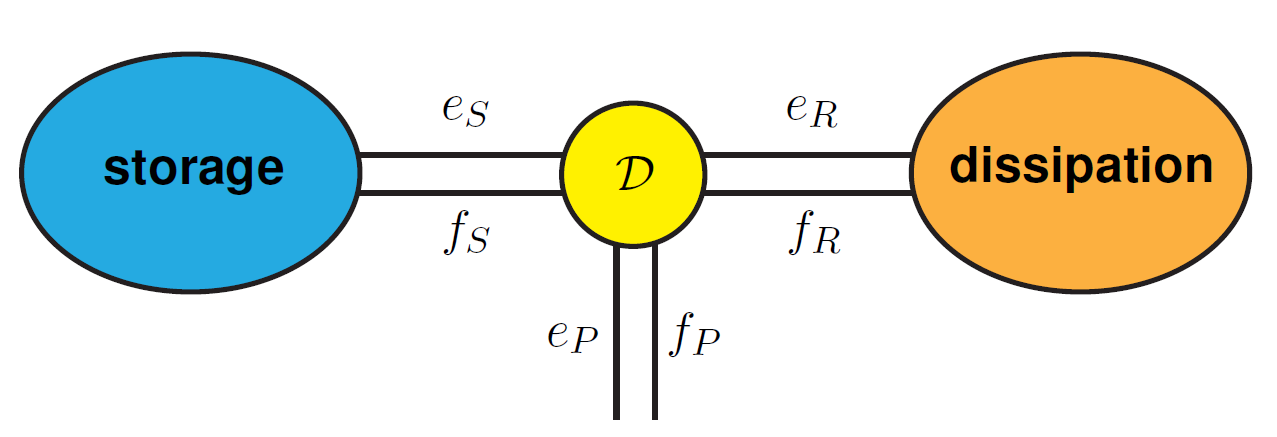
\includegraphics[width=0.6\textwidth]{diracstructure.png}
			\end{figure}
			Elements are geometrically interconnected by the \emph{energy routing} structure $\mathcal{D}$
			\begin{itemize}
				\item Energy storing elements (inertia, spring)
				\item Energy dissipating elements (damper)
				\item Energy conservative elements (transformer, gyrator)
			\end{itemize}
			Energy supply through port $(f_p,e_p)$ from \emph{operator} or \emph{environment}
\end{frame}

%\begin{frame}
%	\frametitle{Energy consistent modelling and control}
%	\begin{itemize}
%		\item \emph{Virtual object} concept
%			\begin{itemize}%[leftmargin=0em]
%  				\renewcommand{\labelitemi}{$\Rightarrow$}
%				\item Maps object forces to manipulators
%				\item Stores kinetic energy
%				\item Changes size to adjust formation
%			\end{itemize}
%		\item Model represents energy content of the complete system
%		\item Dampers dissipate energy: \textbf{passive system}
%		\item Operator controls system by energy supply
%			\begin{block}{Stability}
%Model errors never influence passivity nor stability \cite{Stramigioli_01}
%	\end{block}	
%		\end{itemize}
%%\begin{itemize}%[leftmargin=0em]
%%  \renewcommand{\labelitemi}{$\Rightarrow$}
%%\item enhanced human perception through control of a meaningful quantity and appropriate feedback
%%\item stability over a wide class of environments
%%			\end{itemize}
%%		\begin{quote}
%%		If a controlled robot is not passive there is always a passive environment that destabilizes the interconnected system \cite{Stramigioli_15}
%%		\end{quote}
%
%
%\end{frame}


%\begin{frame}
%	\frametitle{Intrinsically Passive Control (IPC)}
%	\begin{columns}
%		\column{0.4\linewidth}
%			
%	
%		\begin{itemize}
%			\item High-level Supervisor and low-level IPC
%			\item IPC + robot: passive
%			\item Power provided by Supervisor
%			\item Environment assumed passive
%		\end{itemize}
%
%		
%		\column{0.58\linewidth}
%             \begin{figure}[htb]
%			\centering
%			%\psfrag{q1}[Bl][Bl]{\small $\alpha$}
%			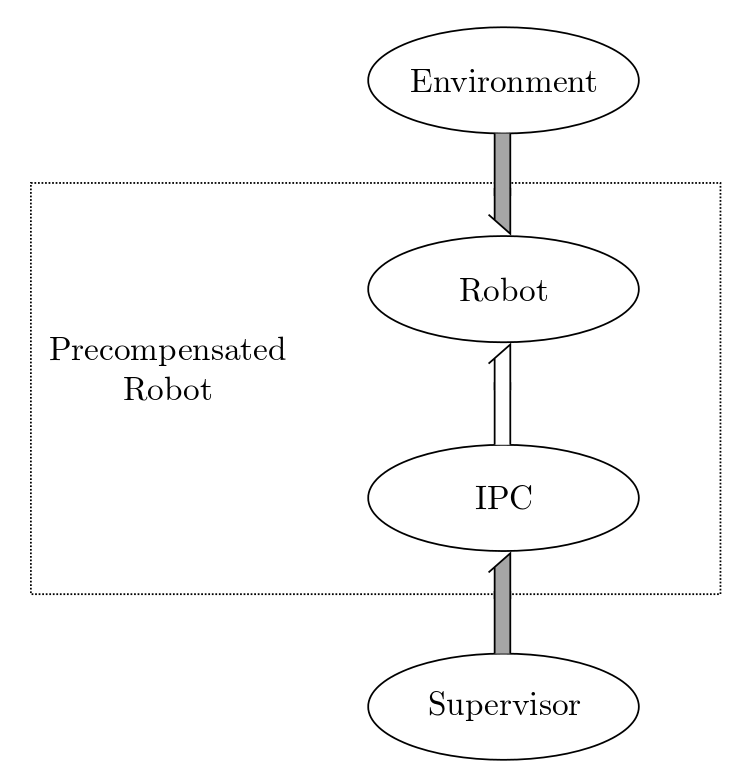
\includegraphics[width=0.9\textwidth]{IPCoverview.png}
%			\caption{Overview of the IPC architecture 								\cite{Stramigioli_01}}
%			\end{figure}
%		
%			
%		\end{columns}
%\end{frame}

\begin{frame}
	\frametitle{System model} \[
	\begin{pmatrix}	\dot{x}_M \\ \dot{x}_S\end{pmatrix} = 
	\begin{pmatrix}J_M & -(\phi_M)^T\\ \phi_M & 0 \end{pmatrix} 
	\begin{pmatrix}\frac{\partial H}{\partial x_M} \\ \frac{\partial H}{\partial x_S}\end{pmatrix}
	+ \begin{pmatrix} 0 & 0 & 0 \\ \phi_h & \phi_{rl} & \phi_m \end{pmatrix}
	\begin{pmatrix}
	T_h \\ T_{rl} \\ T
	\end{pmatrix} \]
	\[ \begin{pmatrix} W_h \\ W_{rl} \\ W \end{pmatrix} = 
	\begin{pmatrix}0 & \phi_h^T \\ 0 & \phi_{rl}^T \\ 0 & \phi_m^T \end{pmatrix}
	\begin{pmatrix}\frac{\partial H}{\partial x_M}\\\frac{\partial H}{\partial x_S}\end{pmatrix} \]

\begin{columns}
		\column{0.5\linewidth}
\begin{itemize}
\item $ x_M$: inertia state vector 
\item $ x_S $: spring state vector
%\item $H = H_S + H_M$: sum of energies
%\item $\phi_M,J_M,\phi_h,\phi_{rl}$: geometric description matrices
\item $T_h$: desired object twist
\item $T_{rl}$: desired rest-length twist
\item $T$: manipulator twist
\item $W_h,W_{rl},W$: wrenches
\end{itemize}

%Reference inputs: $T_h,T_{rl}$\\
%Control output: end-effector wrenches $W_E = -(\phi_E)^T \frac{\partial H}{\partial x_S} $
		\column{0.5\linewidth}

             \begin{figure}[htb]
			\centering
			%\psfrag{q1}[Bl][Bl]{\small $\alpha$}
			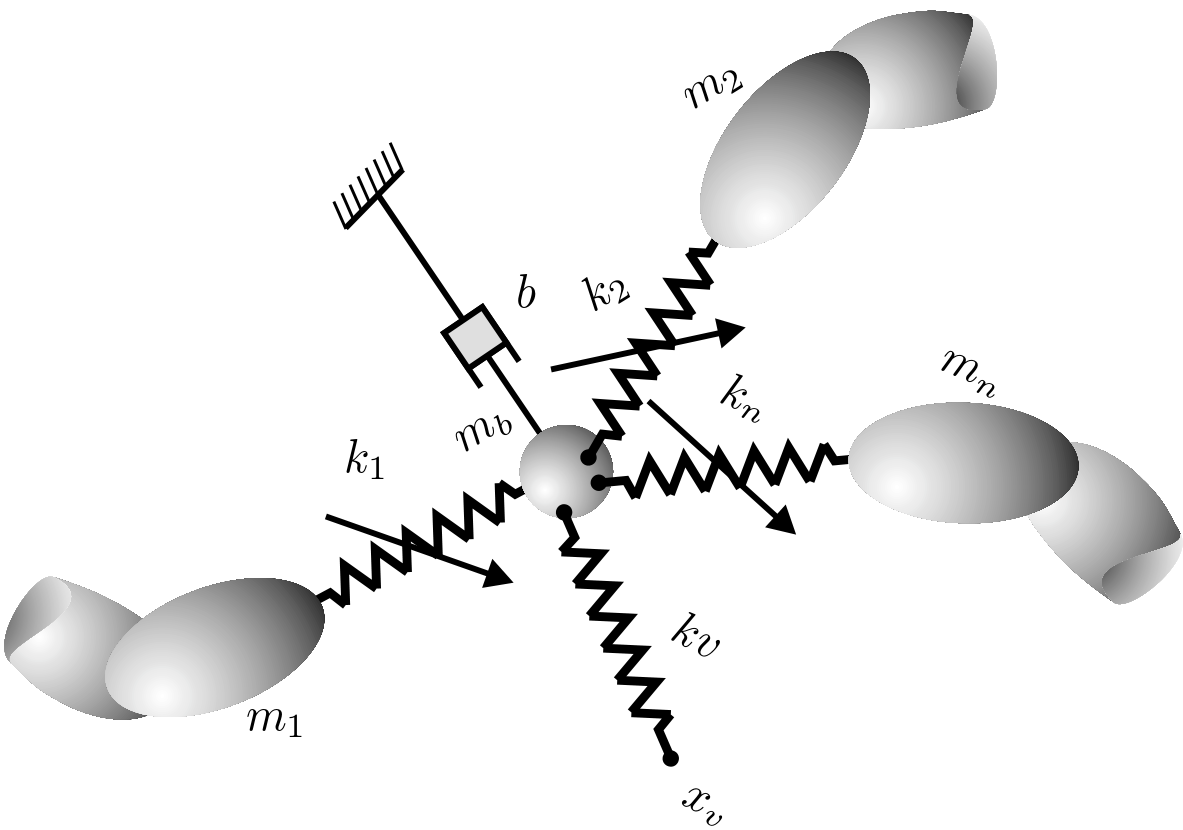
\includegraphics[width=0.9\textwidth]{IPCsprings.png}
			\end{figure}
		\end{columns}

\end{frame}

\begin{frame}
	\frametitle{Intrinsically Passive Control}
	\begin{block}{}
	Control based on the model of an impedance controlled cooperative manipulation set-up
	\end{block}
 \begin{figure}[htb]
 \vspace{-15pt}
			\centering
			%\psfrag{q1}[Bl][Bl]{\small $\alpha$}
			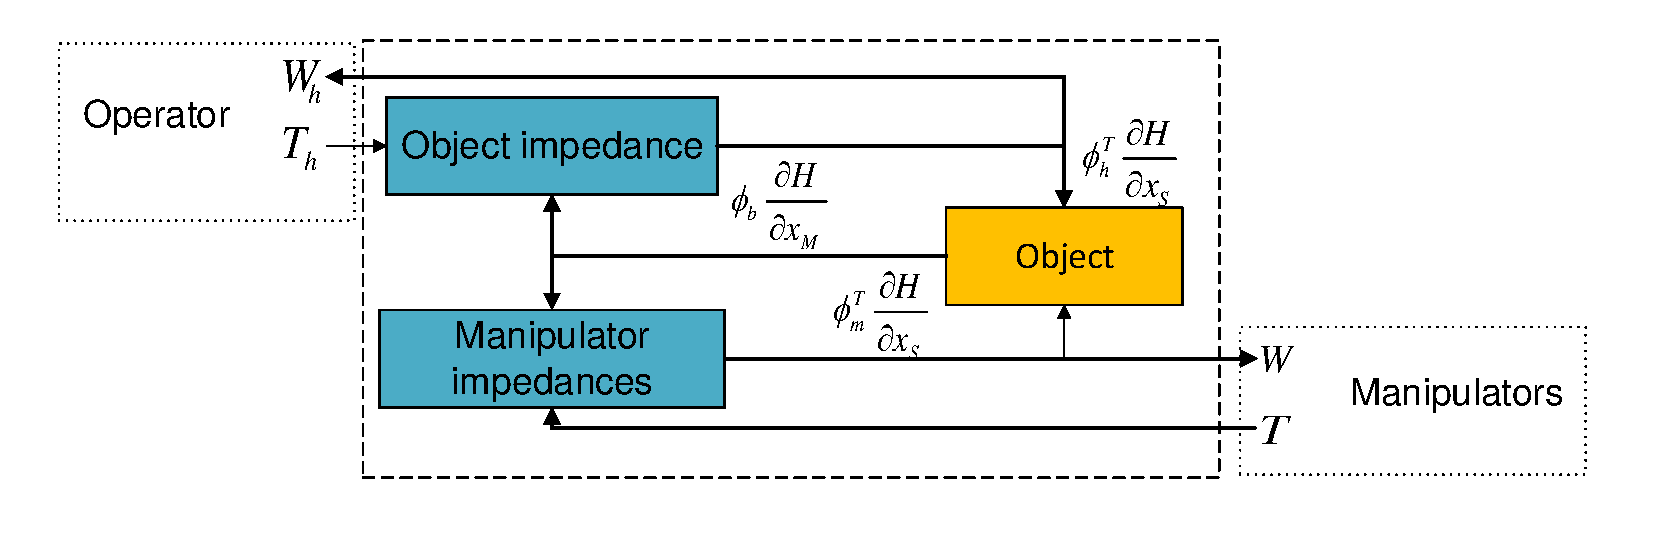
\includegraphics[width=1\textwidth]{IPCscheme.pdf}
\vspace{-30pt}
\end{figure}
\begin{columns}[t]
		\column{1\linewidth}
			
	
		\begin{itemize}
%			\item Geometric interconnection of springs, masses and dampers
			\item Internal and external \emph{impedance} relations
%			\item No manipulator inertia re-shaping + dampers: \textbf{passivity}
			\item Energy supplied by operator/environment
%			\item Formation changes through variable virtual object shape
		\end{itemize}

		
%		\column{0\linewidth}
%             \begin{figure}[htb]
%			\centering
%			%\psfrag{q1}[Bl][Bl]{\small $\alpha$}
%			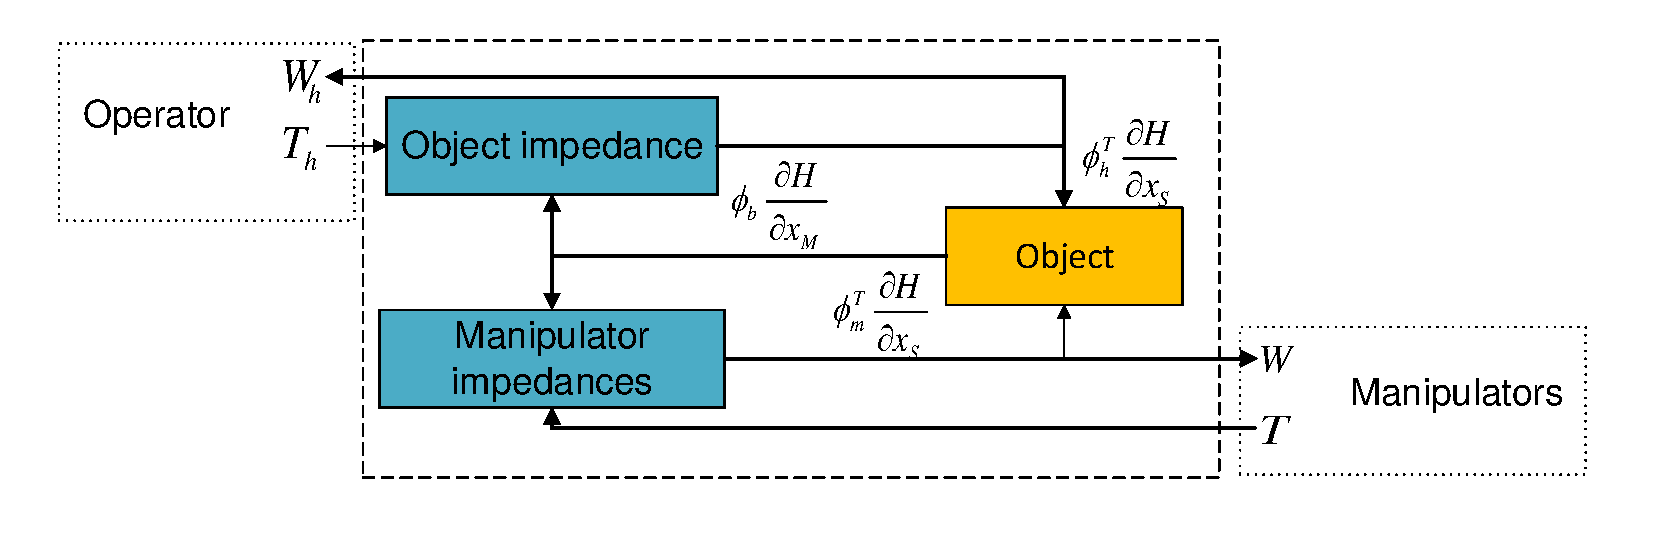
\includegraphics[width=0.98\textwidth]{IPCscheme.pdf}
%
%			\end{figure}
		
			
		\end{columns}
					\begin{block}{Stability}
Model errors never influence passivity nor stability \nocite{Stramigioli_01}{\tiny [Str01]} 
	\end{block}
\end{frame}



%\begin{frame}
%	\frametitle{Grasping an object}
%\begin{columns}
%		\column{0.4\linewidth}
%			
%	
%		\begin{itemize}
%			\item Variable rest-length springs
%			\item Rest-length: virtual object size
%			\item Distinct power port
%		\end{itemize}
%
%		
%		\column{0.62\linewidth}
%             \begin{figure}[htb]
%			\centering
%			%\psfrag{q1}[Bl][Bl]{\small $\alpha$}
%			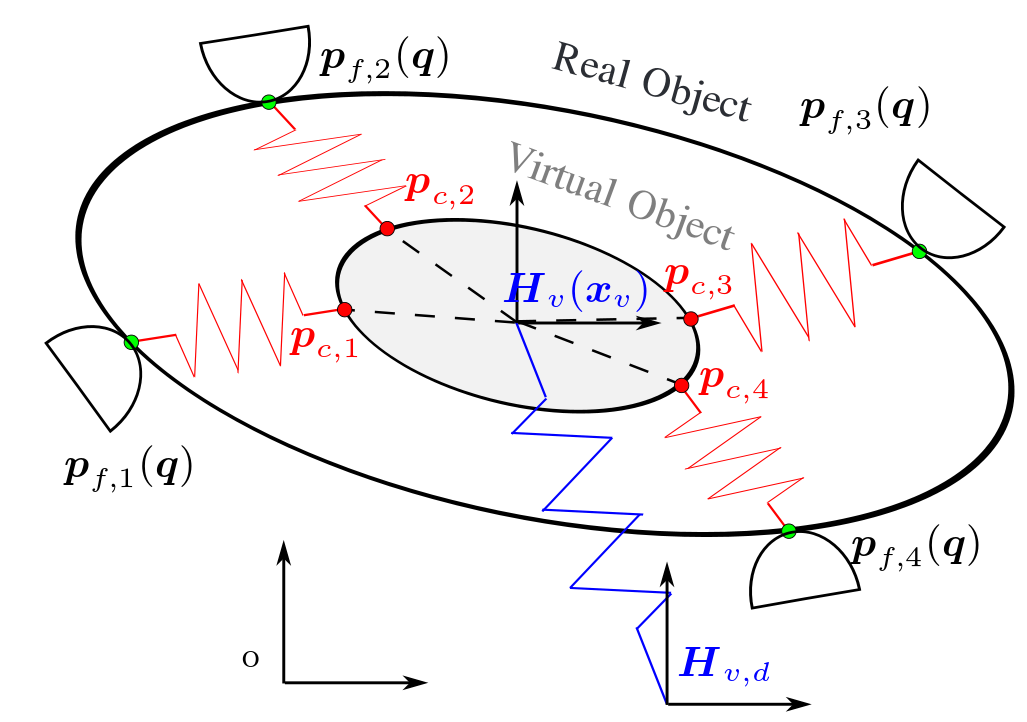
\includegraphics[width=0.98\textwidth]{IPCobjects.png}
%			\caption{Virtual and real object \cite{Wimboeck_08}}
%			\end{figure}
%		
%			
%		\end{columns}
%\end{frame}




%\begin{frame}
%	\frametitle{Future work: Internal force control}
%	Friction constraint of a \emph{soft finger}
%	\[f_N \geq \frac{1}{\mu_f} \vert f_T \vert + \frac{1}{\mu_m} \vert m_N \vert
%	\]
%	\begin{itemize}
%		\item Autonomous control of grasping forces subject to dynamic manipulation requirements
%		\item Energy taken from virtual object spring
%		\item Operator sets constant grasping forces
%	\end{itemize}
%	
%	
%\end{frame}

\section{Results}
%\begin{frame}
%	\frametitle{Grasping force optimization for friction contacts}
%	\begin{columns}
%	\column{0.6\textwidth}
%	\begin{itemize}
%	\item required contact normal force is dependent on tangential forces
%	\item high tangential forces arise during acceleration
%	\item other requirements: safety margin, maximum grasping force $\Rightarrow$ cost function
%	\item linear matrix inequality (LMI) problem
%	\end{itemize}
%	\column{0.5\textwidth}
%
%\begin{figure}[htb]
%			\centering
%			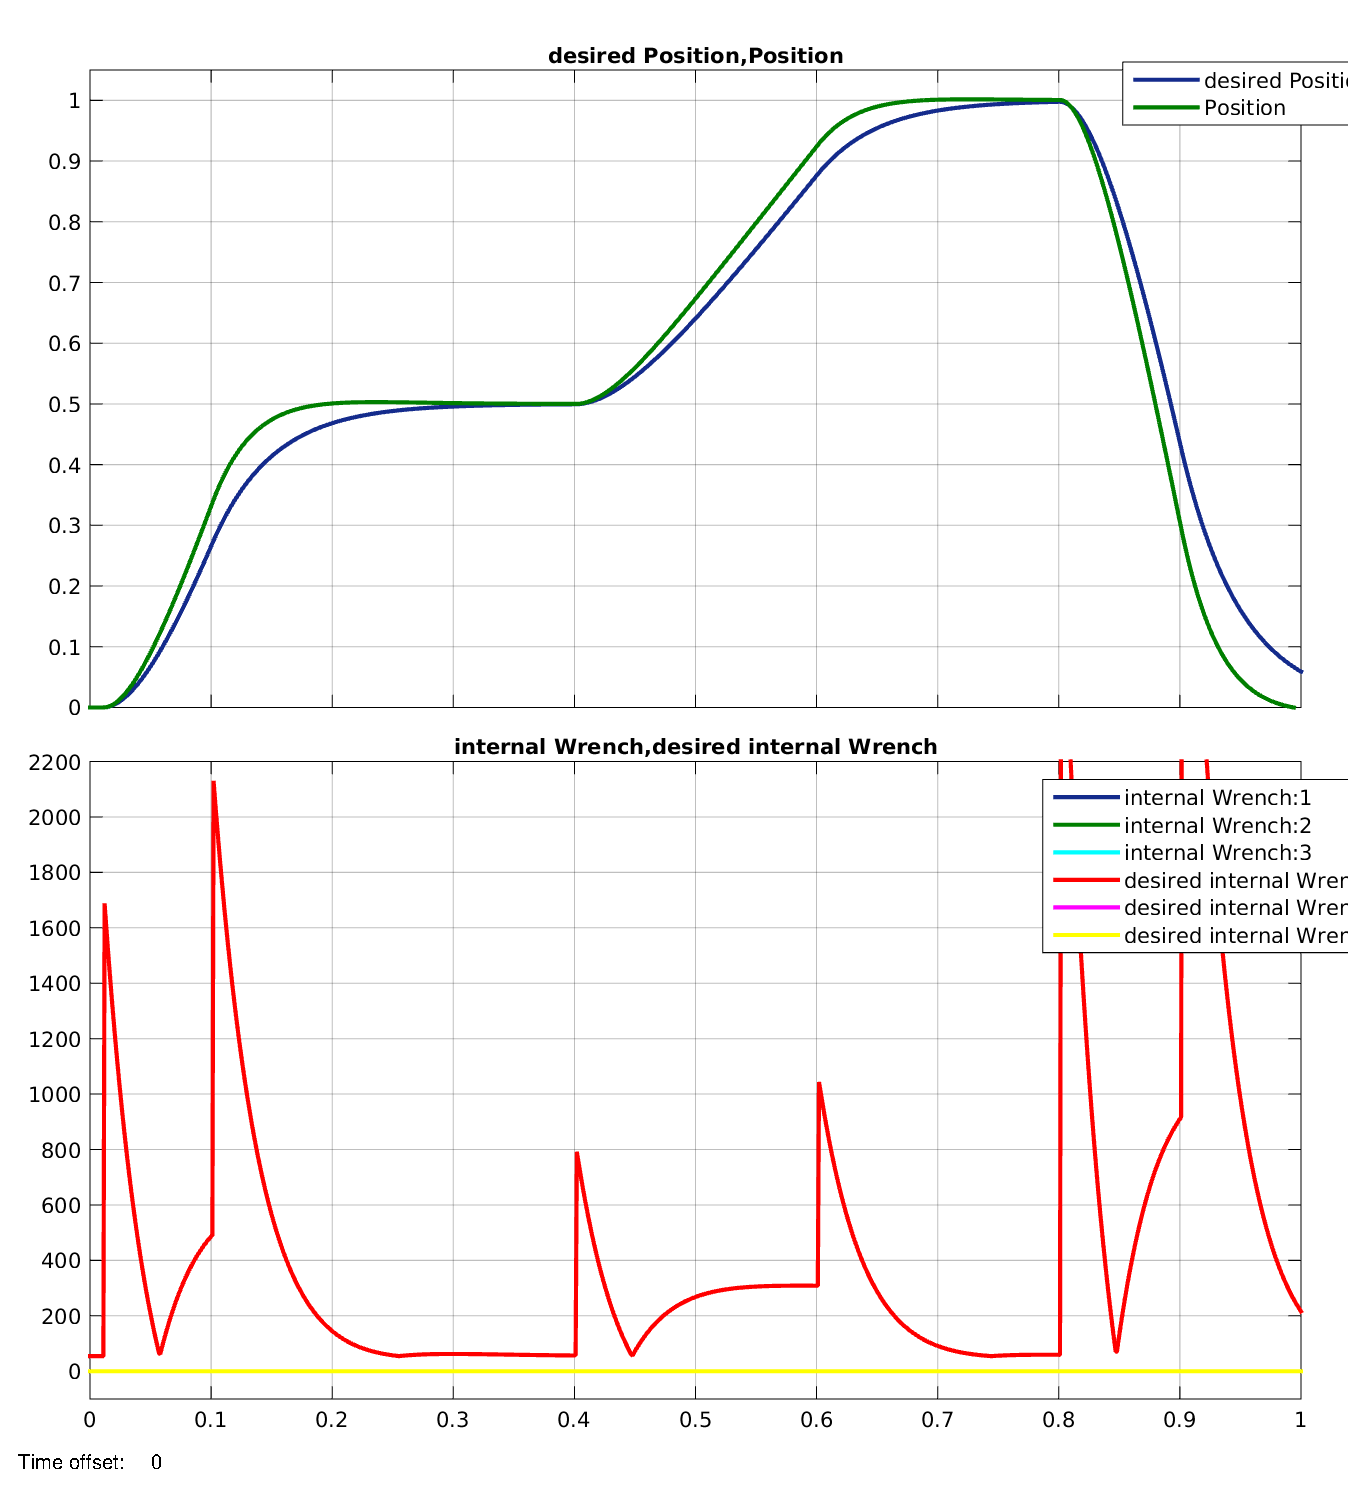
\includegraphics[width=0.9\textwidth]{Hanposforce.eps}
%			\caption{Position, Internal wrench}
%\end{figure}
%\end{columns}
%\end{frame}
\begin{frame}
	\frametitle{Comparison: position tracking}
%Impedance-based reference trajectory generation \cite{Caccavale_01}
\begin{figure}[t]
\begin{tikzpicture}
	\begin{axis} [
		ylabel = {$p_x$[m]},
		xlabel = {t[s]},
		minor y tick num = 1,
		axis lines = left,
		legend entries = {desired position, object force feed-forward, impedance-based trajectory gen., virtual object},
		legend style = {at={(axis cs:1.2, 0.07)}, anchor = north},
		legend cell align=left,
		grid = major,
		height=7.5cm,
		width=0.98\linewidth
	]
\addplot[blue,]
	table {/home/mangerer/MAgit/MA/Latex/plotdata/DePatransdesiredPosition.txt};\addplot[red,]
	table {/home/mangerer/MAgit/MA/Latex/plotdata/DePatransPosition.txt};
\addplot[yellow,]
	table {/home/mangerer/MAgit/MA/Latex/plotdata/CaVi_Position.txt};
\addplot[green,]
	table {/home/mangerer/MAgit/MA/Latex/plotdata/DIPCtransPosition.txt};
\end{axis}
\end{tikzpicture}
%\begin{tikzpicture}
%	\begin{axis} [
%		ylabel = {$p_x$[m]},
%		xlabel = {t[s]},
%		minor y tick num = 1,
%		axis lines = left,
%		legend entries = {position,desired position},
%		legend style = {at={(axis cs:2.6, 0.7)}, anchor = north},
%		legend cell align=left,
%		grid = major,
%		height=3.5cm,
%		width=0.98\linewidth
%	]
%\addplot[red,]
%	table {/home/mangerer/MAgit/MA/Latex/plotdata/DIPCtransPosition.txt};
%\addplot[blue,]
%	table {/home/mangerer/MAgit/MA/Latex/plotdata/DIPCtransdesiredPosition.txt};
%\end{axis}
%\end{tikzpicture}
\vspace{-20pt}
%\caption{Top: Object force feed-forward;
%Bottom: Virtual Object}
\end{figure}
\end{frame}

\begin{frame}
	\frametitle{Comparison: velocity tracking}
%Internal impedance control with object force-feedforward \cite{DePascali_15}
\begin{figure}[t]
\begin{tikzpicture}
	\begin{axis} [
		ylabel = {$v_x$[m/s]},
		xlabel = {t[s]},
		minor y tick num = 1,
		axis lines = left,
		legend entries = {desired velocity, object force feed-forward, impedance-based trajectory gen., virtual object},
		legend style = {at={(axis cs:0.8, -2)}, anchor = north},
		legend cell align=left,
		grid = major,
		height=7.5cm,
		width=0.98\linewidth
	]
\addplot[blue,]
	table {/home/mangerer/MAgit/MA/Latex/plotdata/CaVi_desiredVelocity.txt};
\addplot[red,]
	table {/home/mangerer/MAgit/MA/Latex/plotdata/DePatransVelocity.txt};
\addplot[yellow,]
	table {/home/mangerer/MAgit/MA/Latex/plotdata/CaVi_Velocity.txt};
\addplot[green,]
	table {/home/mangerer/MAgit/MA/Latex/plotdata/DIPCtransVelocity.txt};
\end{axis}
\end{tikzpicture}
%\begin{tikzpicture}
%	\begin{axis} [
%		ylabel = {$v_x$[m]},
%		xlabel = {t[s]},
%		minor y tick num = 1,
%		axis lines = left,
%		legend entries = {velocity,desired velocity},
%		legend style = {at={(axis cs:0.8, -0.5)}, anchor = north},
%		legend cell align=left,
%		grid = major,
%		height=3.5cm,
%		width=0.98\linewidth
%	]
%\addplot[red,]
%	table {/home/mangerer/MAgit/MA/Latex/plotdata/DIPCtransVelocity.txt};
%\addplot[blue,]
%	table {/home/mangerer/MAgit/MA/Latex/plotdata/DIPCtransdesiredVelocity.txt};
%\end{axis}
%\end{tikzpicture}
\vspace{-20pt}
%\caption{Top: External impedance based reference trajectory generation; Bottom: Virtual object}
\end{figure}
\end{frame}

%\begin{frame}
%	\frametitle{Comparison: internal forces (rotation)}
%\begin{figure}[t]
%
%\begin{tikzpicture}
%	\begin{axis} [
%		ylabel = {f[N],m[Nm]},
%		xlabel = {t[s]},
%		minor y tick num = 1,
%		axis lines = left,
%		%legend entries = {force $f_{int,x}$, force $f_{int,y}$, torque $m_{int,z}$},
%		%legend style = {at={(axis cs:2.6, 0.04)}, anchor = north},
%		%legend cell align=left,
%		grid = major,
%		height=3.3cm,
%		width=0.98\linewidth
%	]
%\addplot[red,]
%	table {/home/mangerer/MAgit/MA/Latex/plotdata/DePaIntWrenchtx.txt};
%\addplot[blue,]
%	table {/home/mangerer/MAgit/MA/Latex/plotdata/DePaIntWrenchty.txt};
%	\addplot[green,]
%	table {/home/mangerer/MAgit/MA/Latex/plotdata/DePaIntWrenchrz.txt};\end{axis}
%\end{tikzpicture}
%\begin{tikzpicture}
%	\begin{axis} [
%		ylabel = {f[N],m[Nm]},
%		xlabel = {t[s]},
%		minor y tick num = 1,
%		axis lines = left,
%		legend entries = {force $f_{int,x}$, force $f_{int,y}$, torque $m_{int,z}$},
%		legend style = {at={(axis cs:2.6, 0.1)}, anchor = north},
%		legend cell align=left,
%		grid = major,
%		height=3.3cm,
%		width=0.98\linewidth
%	]
%\addplot[red,]
%	table {/home/mangerer/MAgit/MA/Latex/plotdata/DIPCInternalWrenchtx.txt};
%\addplot[blue,]
%	table {/home/mangerer/MAgit/MA/Latex/plotdata/DIPCInternalWrenchty.txt};
%	\addplot[green,]
%	table {/home/mangerer/MAgit/MA/Latex/plotdata/DIPCInternalWrenchrz.txt};\end{axis}
%\end{tikzpicture}
%\vspace{-28pt}
%\caption{Top: Object force feed-forward;
%Bottom: Virtual Object}
%\end{figure}
%\end{frame}
\section{Conclusion}

\begin{frame}
	\frametitle{Human in the loop}
	\begin{itemize}
			\item Desired object position is connected with a spring to the human
			\item Time-discrete reference changes possibly violate passivity
			\item Spring energy leap $\Delta \bar{P}(k) = H_S(t_k) - H_S(t_k^-)$ 
			\item Pre-filled energy tank to allow for initial twist
%			\item Passive Set Position Modulation \cite{Lee_10}
%			\item Suitable for bilateral tele-manipulation
%			\item Spring rest-lengths: adjust to grasp/release objects
		\end{itemize}
		\begin{figure}
					\centering
					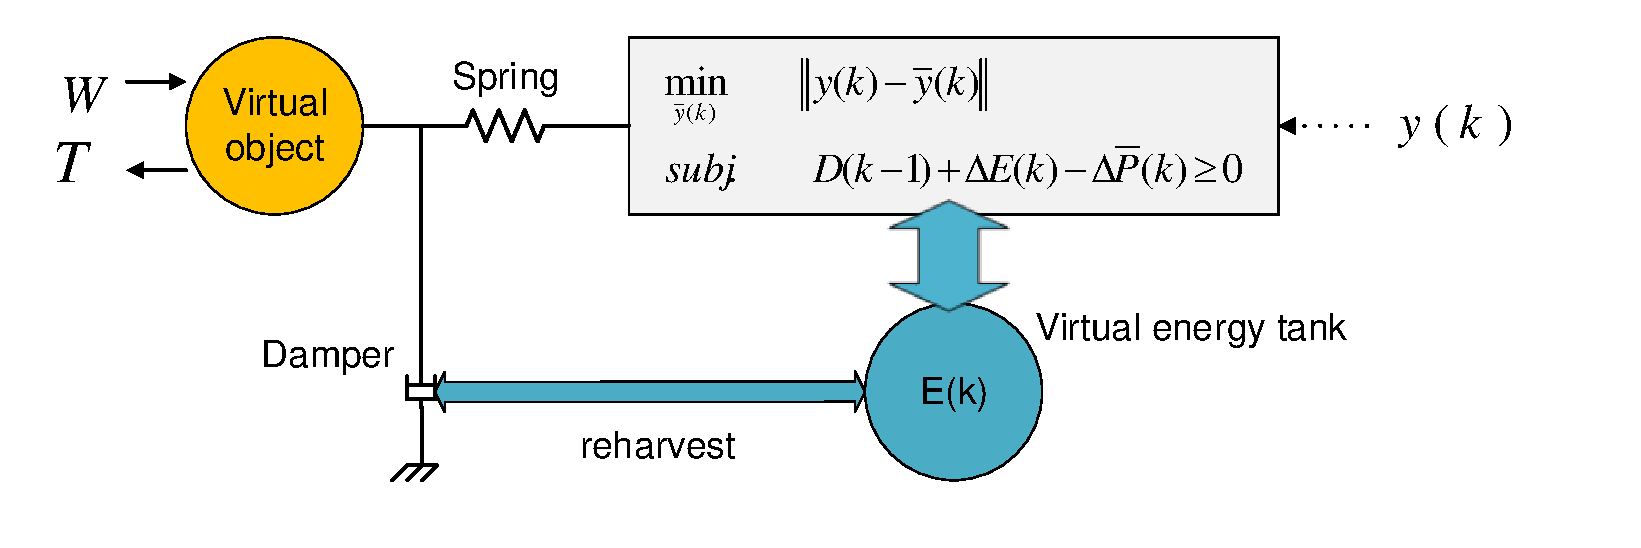
\includegraphics[width=1\textwidth]{pspm.pdf}

		\end{figure}
\end{frame}

\begin{frame}
	\frametitle{Overview \& open issues}
	\begin{itemize}
		\item port-Hamiltonian model of a cooperative manipulation set-up
		\item Appropriate dynamic performance of the model-based controller

  
	\end{itemize}
		\begin{block}{Open issues}
\begin{itemize}
\item Formulation of the HIL in the Hamiltonian framework
\item Passive, stable closed loop behaviour
\item Experimental evaluation
\end{itemize}
	\end{block}	
\end{frame}
\appendix
%\nocite{buss11}
%\nocite{bauer09}
\begin{frame}[allowframebreaks]
	\frametitle{References}
	%\tiny
	%\bibliographystyle{plain}
	%\bibliography{ref}
	\printbibliography
\end{frame}


\end{document}
